\section{Réciproque du théorème de Thalès}
    \subsection{Énoncé}
        \begin{theoreme}[\admis]
            Si dans une configuration géométrique :
            \begin{itemize}
                \item Deux droites $(d)$ et $(d')$ sont sécantes en un point $A$.
                \item $B$ et $M$ sont deux points de la droites $(d)$, distincts de A.
                \item $C$ et $N$ sont deux points de la droite $(d')$, distincts de $A$.
                \item Les points $A, M, B$ sont alignés dans le même ordre que les points $A, N, C$.
                \item $\dfrac{AM}{AB} = \dfrac{AN}{AC}$.                
            \end{itemize}
            \medskip
            alors les droites $(BC)$ et $(MN)$ sont parallèles.
        \end{theoreme}

    \subsection{Exemple de rédaction}

        \begin{methode*1}[Justifier que deux droites sont parallèles]
            \begin{multicols}2
                \begin{itemize}
                    \item Déterminer les droites sécantes.                    
                    \item Identifier les deux triangles.
                    \item Vérifier l'ordre d'alignement des points.
                    \columnbreak
                    \item Calculer les rapports de longueurs correspondantes non portées par les droites candidates.                    
                    \item Invoquer la réciproque du théorème de Thalès.
                \end{itemize}
            \end{multicols}

            \exercice

            \begin{minipage}{8cm}
                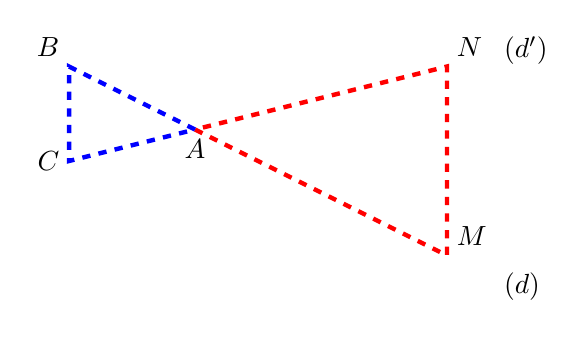
\begin{tikzpicture}[scale = 0.4]
                    \begin{scope}[rotate=90]
                    % \draw[help lines, color=black!30, dashed] (0,0) grid (12,18);        
                    \coordinate[label=below:$A$] (A) at (7,13);
                    \coordinate[label=right:$(d')$] (d') at (9.5,3.5);
                    \coordinate[label=right:$(d)$] (d) at (2,3.5);
                    \coordinate[label=above right:$N$] (N) at (9,5);
                    \coordinate[label=above right:$M$] (M) at (3,5);
                    \coordinate[label=above left:$B$] (B) at (9,17);
                    \coordinate (M1) at (10,17);
                    \coordinate[label=left:$C$] (C) at (6,17);
                    \coordinate (N1) at (5,17);
        
                    \tkzDrawLine(A,M);
                    \tkzDrawLine(A,N);
                    \tkzDrawLine(M,N);
                    \tkzDrawLine(B,C);
                    \tkzDrawLine(M1,N1);     
                    \draw[dashed, color=red, ultra thick] (A)--(M)--(N)--(A);
                    \draw[dashed, color=blue, ultra thick] (A)--(B)--(C)--(A);
                    \end{scope}
                \end{tikzpicture}
            \end{minipage}
            \begin{minipage}{8cm}
                \begin{itemize}
                    \item Les droites $(d)$ et $(d')$ se coupent en $A$.
                    \item $AB=\Lg{5.4}$ ; $AM=\Lg{9}$.
                    \item $AC=\Lg{7.5}$ ; $AN=\Lg{12.5}$.
                \end{itemize}

                % \vspace*{1cm}
                Démontrer que les droites $(MN)$ et $(BC)$ sont parallèles.
            \end{minipage}
            
            \correction
            Dans la configuration ci-dessus : 
            \begin{itemize}
                \item les droites $(MB)$ et $(CN)$ sont sécantes en $A$.                
                \item les deux triangles de la configurations sont \textcolor{red}{$AMN$} et \textcolor{blue}{$ABC$}.
                \item Les points $A, M, B$ sont alignés dans le même ordre que les points $A, N, C$.
                \medskip
                \item D'une part $\dfrac{\textcolor{blue}{AB}}{\textcolor{red}{AM}} = \dfrac{\textcolor{blue}{5,4}}{\textcolor{red}{9}}=0,6$
                \hfill
                D'autre part $\dfrac{\textcolor{blue}{AC}}{\textcolor{red}{AN}} = \dfrac{\textcolor{blue}{7,5}}{\textcolor{red}{12,5}}=0,6$
            \end{itemize}
            On constate que $\dfrac{AM}{AB} = \dfrac{AN}{AC}$, d'après la réciproque du théorème de Thalès, on peut conclure que \psshadowbox{les droites $(MN)$ et $(BC)$ ne sont pas parallèles}.
        \end{methode*1}